% \VignetteEngine{knitr::knitr}
\documentclass{bmcart}\usepackage[]{graphicx}\usepackage[]{color}
%% maxwidth is the original width if it is less than linewidth
%% otherwise use linewidth (to make sure the graphics do not exceed the margin)
\makeatletter
\def\maxwidth{ %
  \ifdim\Gin@nat@width>\linewidth
    \linewidth
  \else
    \Gin@nat@width
  \fi
}
\makeatother

\definecolor{fgcolor}{rgb}{0.345, 0.345, 0.345}
\newcommand{\hlnum}[1]{\textcolor[rgb]{0.686,0.059,0.569}{#1}}%
\newcommand{\hlstr}[1]{\textcolor[rgb]{0.192,0.494,0.8}{#1}}%
\newcommand{\hlcom}[1]{\textcolor[rgb]{0.678,0.584,0.686}{\textit{#1}}}%
\newcommand{\hlopt}[1]{\textcolor[rgb]{0,0,0}{#1}}%
\newcommand{\hlstd}[1]{\textcolor[rgb]{0.345,0.345,0.345}{#1}}%
\newcommand{\hlkwa}[1]{\textcolor[rgb]{0.161,0.373,0.58}{\textbf{#1}}}%
\newcommand{\hlkwb}[1]{\textcolor[rgb]{0.69,0.353,0.396}{#1}}%
\newcommand{\hlkwc}[1]{\textcolor[rgb]{0.333,0.667,0.333}{#1}}%
\newcommand{\hlkwd}[1]{\textcolor[rgb]{0.737,0.353,0.396}{\textbf{#1}}}%

\usepackage{framed}
\makeatletter
\newenvironment{kframe}{%
 \def\at@end@of@kframe{}%
 \ifinner\ifhmode%
  \def\at@end@of@kframe{\end{minipage}}%
  \begin{minipage}{\columnwidth}%
 \fi\fi%
 \def\FrameCommand##1{\hskip\@totalleftmargin \hskip-\fboxsep
 \colorbox{shadecolor}{##1}\hskip-\fboxsep
     % There is no \\@totalrightmargin, so:
     \hskip-\linewidth \hskip-\@totalleftmargin \hskip\columnwidth}%
 \MakeFramed {\advance\hsize-\width
   \@totalleftmargin\z@ \linewidth\hsize
   \@setminipage}}%
 {\par\unskip\endMakeFramed%
 \at@end@of@kframe}
\makeatother

\definecolor{shadecolor}{rgb}{.97, .97, .97}
\definecolor{messagecolor}{rgb}{0, 0, 0}
\definecolor{warningcolor}{rgb}{1, 0, 1}
\definecolor{errorcolor}{rgb}{1, 0, 0}
\newenvironment{knitrout}{}{} % an empty environment to be redefined in TeX

\usepackage{alltt}

\usepackage{xcolor}
\usepackage{url}
\usepackage{amsmath}
\usepackage{amsthm}
\usepackage{amssymb}
\usepackage{graphicx}
\usepackage{tikz}
\usetikzlibrary{shapes,arrows}
\usepackage{float}
\usepackage{verbatim}
\usepackage{hyperref}
\hypersetup{
     colorlinks   = true,
     citecolor    = black
}
\hypersetup{linkcolor=black}
% \hypersetup{linkcolor=black}
% \hypersetup{linkcolor=black}

\usepackage{wrapfig}


% \usepackage{authblk}
\usepackage[utf8]{inputenc} %unicode support

\newcommand{\sig}{\sigma^{70}}
\IfFileExists{upquote.sty}{\usepackage{upquote}}{}
\begin{document}

%\maketitle


\begin{frontmatter}

\begin{fmbox}
\dochead{Draft}

\title{Data exploration, quality control and statistical analysis of
  ChIP-exo experiments}

\author[
   addressref={aff6},                   % id's of addresses, e.g. {aff1,aff2}
   email={chungd@musc.edu}   % email address
]{\inits{DC}\fnm{Dongjun} \snm{Chung}}
\author[
   addressref={aff1},
   email={welch@stat.wisc.edu}
]{\inits{RW}\fnm{Rene} \snm{Welch}}
\author[
   addressref={aff3},
   email={ong@cs.wisc.edu}
]{\inits{IO}\fnm{Irene} \snm{Ong}}
\author[
   addressref={aff3,aff4},
   email={jagrass@wisc.edu}
]{\inits{JG}\fnm{Jeffrey} \snm{Grass}}
\author[
   addressref={aff3,aff4,aff5},
   email={landick@bact.wisc.edu}
]{\inits{RL}\fnm{Robert} \snm{Landick}}
\author[
   addressref={aff1,aff2},
   corref={aff1},
   email={keles@stat.wisc.edu}
]{\inits{SK}\fnm{S\"und\"uz} \snm{Kele\c{s}}}


\address[id=aff1]{%                           % unique id
  \orgname{Department of Statistics, University of Wisconsin Madison}, % university, etc
  \street{1300 University Avenue},                     %
  %\postcode{}                                % post or zip code
  \city{Madison},                              % city
  \cny{WI}                                    % country
}

\address[id=aff2]{%
  \orgname{Department of Biostatistics and Medical Informatics, University of Wisconsin Madison},
  \street{600 Highland Avenue},
%  \postcode{24105}
  \city{Madison},
  \cny{WI}
}
\address[id=aff3]{
  \orgname{Great Lakes Bioenergy Research Center, University of Wisconsin Madison},
  \street{1552 University Avenue},
  \city{Madison},
  \cny{WI}
}
\address[id=aff4]{
  \orgname{Department of Biochemistry, University of Wisconsin Madison},
  \street{433 Babcock Drive},
  \city{Madison},
  \cny{WI}
}
\address[id=aff5]{
  \orgname{Department of Bacteriology, University of Wisconsin Madison},
  \street{1550 Linden Drive},
  \city{Madison},
  \cny{WI}
}
\address[id=aff6]{
  \orgname{Department of Public Health Sciences, Medical University of South Carolina},
  \street{135 Cannon Street},
  \city{Charleston},
  \cny{SC}
}


% \begin{artnotes}
% %\note{Sample of title note}     % note to the article
% \note[id=n1]{Equal contributor} % note, connected to author
% \end{artnotes}


\end{fmbox}

\begin{abstractbox}

  \begin{abstract}

    ChIP-exo is a modification of the ChIP-Seq protocol for high
    resolution mapping of transcription factor binding sites. Although
    many aspect of the ChIP-exo data analysis are similar to those of
    ChIP-Seq, ChIP-exo presents a number of unique challenges. We
    present a quality control pipeline that analyzes a ChIP-exo
    experiment's strand imbalance, enrichment and library
    complexity. Assessment of these characteristics are facilitated
    through diagnostic plots and summary statistics calculated over
    regions of the genome with varying levels of coverage.

    We systematically evaluated diverse aspects of ChIP-exo and found
    the following characteristics: First, ChIP-exo's background is
    quite different from ChIP-Seq's. Second, although often assumed in
    ChIP-exo data analysis methods, the ``peak pair'' assumptions does
    not hold locally in actual ChIP-exo data. Third, we for the first
    time compared Paired End (PE) ChIP-Seq with ChIP-exo and found
    that both protocols are comparable in resolutions and sensitivity
    for closely located binding events, but as the distance between
    binding events increases ChIP-exo shows higher sensitivity that PE
    ChIP-Seq. Finally, at fixed sequencing depths, ChIP-exo provides
    higher sensitivity, specificity and spatial resolution than PE
    ChIP-Seq.

  \end{abstract}

\begin{keyword}
  \kwd{ChIP-exo}
  \kwd{QC}
  \kwd{TFBS}
  \kwd{BS identification on High-Res}
\end{keyword}

\end{abstractbox}

\end{frontmatter}

\newpage

\section{Background}
\label{sec:intro}

ChIP-exo (Chromatin Immunoprecipitation followed by exonuclease
digestion and next generation sequencing) Rhee and Pugh, 2011
\cite{exo1} is the state-of-the-art experiment developed to attain
single base-pair resolution of protein binding site identification and
it is considered as a powerful alternative to popularly used ChIP-Seq
(Chromatin Immunoprecipitation coupled with next generation
sequencing) assay. ChIP-exo experiments first capture millions of DNA
fragments (150 -250 bp in length) that the protein under study
interacts with using random fragmentation of DNA and a
protein-specific antibody. Then, exonuclease is introduced to trim the
5' end of each DNA fragment to a fixed distance from the bound protein
compared to ChIP-Seq. This step is unique to ChIP-exo and could
potentially provide significantly higher spatial resolution compared
to ChIP-Seq. Finally, high throughput sequencing of a small region (25
to 100 bp) at the 5' end of each fragment generates millions of reads.

While the number of ChIP-exo data keeps increasing,characteristics of
ChIP-exo data are not fully investigated yet. First, DNA libraries
generated by the ChIP-exo protocol seem to be less complex than the
libraries generated by ChIP-Seq (Mahony et al., 2015,
\cite{exo_review}), i.e. the possible number of positions to which the
reads can be aligned has been reduced due to the exonuclease
digestion. Second, although there are roughly the same amount of read
in both strands, locally there may be more reads in one strand than in
the other. To address this challenges, we suggest a collection of
quality control visualizations to understand which of this biases are
present in a ChIP-exo experiment and globally asses the enrichment and
library complexity of a ChIP-exo sample. We gathered ChIP-exo data
from diverse organisms: CTCF factor in human \cite{exo1}; ER factor in
human and FoxA1 factor in mouse (Serandour et al., 2013
\cite{exoillumina}); GR in IMR90, K562 and U20S cell lines (Starick et
al., 2015 \cite{starick15}) and generated $\sig$ factor in Escherichia
Coli (\emph{E. Coli}) under aerobic ($ + O_2$) condition, and treated
by rifampicin by 0 and 20 minutes (courtesy of Professor Robert
Landick's lab). %% note to self, we may add more experiments here

Most of current ChIP-Seq quality control (QC) guidelines (Landt et
al., \cite{encode_qc}) may not be applicable on ChIP-exo, additionally
to our knowledge there are not established QC pipelines for
ChIP-exo. Previous ChIP-exo analyses used ChIP-Seq samples to compare
the resolution between experiments (\cite{exo1}, \cite{exo2},
\cite{exoillumina}); Carroll et al., 2014 \cite{carroll.qc} studied
the use of the Strand-Cross Correlation (SCC) (Kharchenko et al., 2008
\cite{strandcc}) and showed that by filtering blacklisted regions the
estimation of the SCC is improved. However, using the SCC may not be
helpful since the peaks that are attained at the read and fragment
lengths are confused in a typical ChIP-exo SCC curve. Additionally
this method requires to know blacklisted regions in advance which may
not be available. In our pipeline we propose an out-the-shelf analysis
that contrasts the enrichment of the experiment against its library
complexity.

In order to obtain the potential benefits of ChIP-exo on protein
binding site identification, it is critical to understand which are
the important characteristics of ChIP-exo data and to use algorithms
that could fully utilize information available in ChIP-exo data. Rhee
and Pugh, 2011 \cite{exo1} discussed that reads in the forward and
reverse strand might construct peak pairs around bound proteins, of
which heights were implicitly assumed to be symmetric. Hence, they
used the ``peak pair method'' that predicts the midpoint of two modes
of peak pairs as potential binding sites. Mace (Wang et al, 20114
\cite{mace}), CexoR (Madrigal, 2015 \cite{cexor}) and Peakzilla
(Bardet et al., 2013 \cite{peakzilla}), recently developed ChIP-exo
data analysis methods are also based on this peak pair
assumption. However, appropriateness of such assumption was not fully
evaluated in the literature yet. Furthermore, it is still unknown
which factors could affect protein binding site identification using
ChIP-exo data. In order to address this problem, we investigated
various aspects of ChIP-exo data by contrasting them with their
respective ChIP-Seq experiments.

Currently, research on statistical methods for ChIP-exo data is still
in its very early stage. Although many methods have been proposed to
identify protein binding sites from ChIP-Seq data (reviewed by
Wilbanks and Facciotti, 2012 \cite{evaluation} and Pepke and Wold,
2009 \cite{computation}), such as MACS (Zhang et al., 2008
\cite{macs}), CisGenome (Ji et al., 2008 \cite{cisgenome}) and MOSAiCS
(Kuan et al., 2009 \cite{mosaics}), these approaches reveal protein
binding sites in lower resolution, i.e., at an interval of hundreds to
thousands of base pairs. Furthermore, they report only one ``mode'' or
``predicted binding location'' per peak. Hence, these methods are not
appropriate to evaluate the potential of ChIP-exo data for high
resolution identification of protein binding sites. More recently,
deconvolution algorithms such as Deconvolution (Lun et al., 2009
\cite{csdeconv}), GEM (Guo et al., 2012 \cite{gem}, an improved
version of Guo et al., 2010 \cite{gps} ) and PICS (Zhang et al., 2010
\cite{pics}) have been proposed to identify binding sites in higher
resolution using ChIP-Seq data. However, most of them are still not
tailored for ChIP-exo and PE and SE ChIP-Seq data in a unified
framework and as a result, currently available methods are not
appropriate for fair comparison between ChIP-exo and ChIP-Seq. To
address these limitations, we developed an improved of dPeak (Chung et
al., 2013 \cite{dpeak}), a high resolution binding site identification
(deconvolution) algorithm that we previously developed for PE and SE
ChIP-Seq data, so that it can also handle ChIP-exo data. The dPeak
algorithm implements a probabilistic model that accurately describes
the ChIP-exo and ChIP-Seq data generation process.

In this work we demonstrate that the ``peak pair'' assumption of Rhee
and Pugh, 2013 \cite{exo2} does not hold well in real ChIP-exo
data. Furthermore, we found that when we analyze ChIP-exo data from
eukaryotic genomes, it is important to consider sequence biases
inherent to ChIP-exo data, such as mappability and GC content in order
to improve sensitivity and specificity of binding site
identification. We evaluated several methods to identify binding events
and dPeak performs competitively respect to GEM and MACE when
analyzing ChIP-exo data. More importantly, when comparable number of
reads is used for both ChIP-exo and ChIP-Seq , dPeak coupled with
ChIP-exo data provides resolution comparable to PE ChIP-Seq and both
significantly improve the resolution of protein binding identification
compared to SE-based analysis with any of the available methods.

\section{Results and discussion}
\label{sec:results}

\subsection{Deeply sequence E. Coli $\sig$ ChIP-exo and ChIP-Seq data}
 
$\sig$ factor is a transcription initiation factor of housekeeping
genesin E. Coli. In this organism's genomes, many promoters contain
multiple transcription start sites (TSS) and these TSS are often
closely spaced (10 $\sim$ 150 bp). These closely spaced binding sites
are considered to be multiple ``switches'' that differentially
regulate gene expression under diverse growth conditions
\cite{regulondb}. Therefore, investigation of ChIP-exo's potential for
identification and differentiation of closely spaced binding sites are
invaluable for elucidating the transcriptional networks of prokaryotic
genomes.

\subsection{Current ChIP-Seq guidelines and quality metrics on ChIP-exo data}

We started our exploration by investigating the suitability of the
current state-of-the-art QC pipelines for ChIP-Seq for ChIP-exo. Table
\ref{tab:qc} contains measures that are commonly calculated for
ChIP-Seq samples: PCR Bottleneck Coefficient (PBC) and the Normalized
Strand Cross-Correlation (NSC) are calculated as in \cite{encode_qc}.
Additionally, we calculated the Forward Strand Ratio (FSR) to compare
the number of fragments sequenced from each strand.

%% We can observe that the PBC is low, hence it would be incorrectly
%% suggested to repeat the experiment.

\begin{table}[h!]
%% need to fix format
  \centering

\begin{knitrout}
\definecolor{shadecolor}{rgb}{0.969, 0.969, 0.969}\color{fgcolor}\begin{kframe}
\begin{verbatim}
##     Organism  IP/TF Condition/Cell Rep.     Depth        PBC        NSC
##  1:   E.Coli  Sig70        Aerobic    1  13961493 0.13994203 103.423876
##  2:   E.Coli  Sig70        Aerobic    2  14810838 0.16339252 162.800188
##  3:   E.Coli  Sig70      Anaerobic    1  16108774 0.13535422 153.508809
##  4:   E.Coli  Sig70      Anaerobic    2  13636541 0.15322537 172.581549
##  5:   E.Coli  Sig70       Rif-0min    1    902921 0.26895580  13.769077
##  6:   E.Coli  Sig70       Rif-0min    1   1852124 0.25908459  17.918825
##  7:   E.Coli  Sig70      Rif-20min    2   2104427 0.25841987  29.608305
##  8:   E.Coli  Sig70      Rif-20min    2  11548572 0.15107930  13.086255
##  9:    Human   CTCF           HeLA    1  48478450 0.45796889  16.024817
## 10:    Mouse Fox A1    Mouse Liver    1  22210461 0.65622704  21.281972
## 11:    Mouse Fox A1    Mouse Liver    2  23307557 0.79962169  60.421912
## 12:    Mouse Fox A1    Mouse Liver    3  22421729 0.10683407  72.042428
## 13:    Human     GR          IMR90    1  47443803 0.29785605   8.860176
## 14:    Human     GR           K562    1 116518000 0.05047634   4.117883
## 15:    Human     GR           U20S    1   3255111 0.77142141  10.058834
## 16:    Human     ER          MCF-7    1   9289835 0.80825680  19.875232
## 17:    Human     ER          MCF-7    2  11041833 0.80241200  21.485094
## 18:    Human     ER          MCF-7    3  12464836 0.82035947  18.728062
\end{verbatim}
\end{kframe}
\end{knitrout}
\caption{Usual quality control indicators applied to the gathered
  ChIP-exo samples.  PBC stands for PCR Bottleneck Coefficient (0 -
  0.5 is severe bottlenecking, 0.5 - 0.8 is moderate bottlenecking,
  0.8 - 0.9 is mild bottlenecking, while 0.9 - 1 is no bottlenecking),
  NSC for Normalized Strand Cross-Correlation and FSR for Forward
  Strand Ratio. We omitted the Relative Strand Cross-Correlation (RSC)
  because a typical ChIP-exo experiment is not accompanied by an input
  file. $\sig$ samples were given by Dr. Landick's Lab, FoxA1 and ER
  samples are from Serandour et al., 2013 \cite{exoillumina} and CTCF
  sample is from Rhee and Pugh, 2011 \cite{exo1}}
  \label{tab:qc} %% need to make this table
\end{table}

It is of special importance to notice that the values of PBC are quite
low, hence it would be necessary to repeat these experiments by
following ChIP-seq guidelines. On the other hand, in a good ChIP-Seq
experiment the SCC is maximized at the fragment length, and a
``phantom peak'' would be also present at the experiment's read length
(\cite{encode_qc} and \cite{strandcc}). However, in ChIP-exo's case
these two peaks are confounded. Hence an enrichment measure based in
SCC such as the NSC is harder to interpret. In Figure
\ref{fig:scc_exo} we observe that both local maxima are hard to
differentiate in the SCC curves for the $\sig$ ChIP-exo datasets used to
calculate the NSC values in Table \ref{tab:qc}.

% % According to ENCODE's quality metrics, NSC values close
% % to one corresponds to low enrichment samples or bad quality datasets


\subsection{Comparison with ChIP-Seq data}



We first compared various factors that could affect binding site
identification between ChIP-exo and ChIP-Seq data. In order to compare
distribution of signal and background between ChIP-exo and ChIP-Seq
data, we calculated ChIP tag counts across the genome by counting the
number of reads mapping to each of 150 non-overlapping
window after extending reads by 150 to their 3' end
directions. ChIP tag counts in ChIP-exo data were linearly related to
ChIP tag counts in ChIP-Seq data for the regions with high ChIP tag
counts (Figure \ref{fig:comp}A). This implies that signals for
potential binding sites are well reproducible between ChIP-exo and
ChIP-Seq data. On the other hand, there was clear difference in the
background distribution between them. In ChIP-Seq data reads were
almost uniformly distributed over background (non-binding) regions and
the ChIP tag counts in there regions were significantly larger than
zero. In contrast, in ChIP-exo data, there was larger variation in
ChIP tag counts among background regions and ChIP tag counts were much
lower in these regions compared to ChIP-Seq data. There were also
large proportion of regions without any read in ChIP-exo data. These
results indicate that for ChIP-exo data a much smaller portion of the
genome is expected to be background.

We next evaluated the ``peak pair'' assumption from Rhee and Pugh,
2011 \cite{exo1}, i.e. a peak of reads in the forward strand is
usually paired with a peak of reads in the reverse strand that is
located in the other site of the binding site. Wang et al., 2014
\cite{mace}, Madrigal 2015 \cite{cexor} and Bardet et al., 2013
\cite{peakzilla} proposed method rely in this assumption. In order to
evaluate this assumption, we reviewed the proportion of reads in the
forward strand in candidate regions (i.e. regions with at least one
binding site) in $\sig$ ChIP-exo data. We found that strands of reads
were much less balanced in ChIP-exo data than in ChIP-Seq data in
these regions with potential binding sites (Fig. \ref{fig:comp}B) and
this indicates that the peak pair assumption might not hold in real
ChIP-exo data.

We evaluated ChIP-exo data for CTCF factor from human genome
\cite{exo1} to investigate issues specific to eukaryotic genomes for
binding sites identification. Figures \ref{fig:comp}C and
\ref{fig:comp}D display the bin-level average read counts against
mappability and GC content. Each data point is obtained by averaging
the read counts across bins with the same mappability of GC
content. These results indicate that binding site identification in
ChIP-exo sample might also benefit from the use of methods that take
into account of apparent sequence biases such as mappability and GC
content.


\subsection{ChIP-exo Quality Control Pipeline}

Figure \ref{fig:qcdiagram} shows a flowchart for the ChIP-exo QC
pipeline. Which basically partitions the genome by keeping the
non-digested ChIP-exo regions. Then, for each region calculates a
series of summary statistics. Finally it creates several
visualizations designed to diagnose the quality level of ChIP-exo
sample.

\subsubsection{Enrichment and library complexity in ChIP-exo data}

In ChIP-exo experiments, the background is often digested by the
exonuclease enzyme, therefore to determine the sample's quality is
necessary to address the balance between the enrichment and library
complexity of an experiment. To diagnose this, we considered the
Average Read Coverage (ARC) and the Unique Read Coverage Rate (URCR)
which are defined as follows:

\begin{align*}
  \text{ARC} &= \dfrac{\text{Nr. of reads in the region}}{\text{Width of the region}} \\
  \text{URCR} &= \dfrac{\text{Nr. of reads in the region mapped to
      exactly one position}}{\text{Nr. of reads in the region}}
\end{align*}

Using the Fox A1 in mouse liver cell lines from \cite{exoillumina} and
these two quantities, we explored the relationship between library
complexity and experiment enrichment. In Figure \ref{fig:enrich}A we
can observe both statistics for the regions that are common for the
three replicates. This figure shows typical patterns for ChIP-exo
experiment, there are two strong arms: The one on the left with low
ARC and varying URCR corresponds to ChIP-exo's background, usually
regions composed by scattered reads that were not digested during the
exonuclease step; and the one on the right that corresponds to regions
that are usually enriched, for these regions the URCR measures how the
fragments are allocated into the possible positions in a region. Hence
we would expect the first replicate to have have more enriched regions
and the third replicate's library complexity to be lower than the
other two replicates library complexities. To verify this statements,
we extracted the sequences around high confidence binding events and
look for the FoxA1 motif using FIMO \cite{fimo}. Figure
\ref{fig:enrich}B shows the number of candidate regions, which shows
that the first replicate is being allocated into more enriched regions
than the other ones. Figure \ref{fig:enrich}C shows that for the first
and third replicates, the FoxA1 motif is being detected in roughly the
same proportion of sites, and finally in \ref{fig:enrich}D we observe
that the first and third replicate can detect the FoxA1 motif with the
same significance, while the second replicate does not.

\subsubsection{Strand imbalance in ChIP-exo data}

The strand imbalance assessment is based in the observation that the
enriched regions usually are composed of a higher quantity of reads,
therefore we examined the FSR (defined as the ratio of number of
forward stranded reads divided by the total number of reads in a given
region) as the regions with lower depth are being filtered out. This
indicator is of particular importance, since several methods rely on
the ``peak-pair'' assumption. For every ChIP-exo experiment, we
calculated the global FSR and noticed that for all experiments is
roughly $0.5$, which means there are roughly the same amount of reads
in both strands. However figure \ref{fig:strand} shows that the global
FSR does not represent the experiment's local strand imbalance, hence
the ``peak pair'' assumption may not hold well in real ChIP-exo data.

In order to asses the strand imbalance we created the visualization
shown in Figure \ref{fig:strand}: Figure \ref{fig:strand}A presents
the FSR's behavior as the lower depth regions are being filtered out,
while B) shows which percentage of the regions are composed by reads
in both strand or only one (forward or backward). In a good data set,
it would be expected that all quantiles shown to be quickly converging
towards the median (in panel A) or the regions composed of reads in
one strand being made of few fragments (in panel B). For each
replicate, we divided the partitioned regions by asking whether they
overlap a set of high quality ChIP-exo peaks, and then we tested
(using the Wilcoxon rank sum test over an imbalance index) if the
strand imbalance's distribution is the same for both classes. For
regions composed by a higher amount of reads, it is harder to
distinguish their peaks by considering only the strand imbalance,
hence in a better quality ChIP-exo experiment it is easier to
distinguish enriched regions by the amount of reads in both
strands. Additionally we may consider that the background of a
ChIP-exo experiment it is more unbalanced than the enriched regions.

\subsection{Comparison with ChIP-Seq data using dPeak}



Figure \ref{fig:reso_all} shows different comparisons among ChIP-exo,
PE ChIP-Seq and SE ChIP-Seq. A RegulonDB annotation (Salgado et al,
2012 \cite{regulondb}) was considered identified if the distance
between it and a dPeak binding site estimate was at most of
$20$ bp. That way, the sensitivity is defined as the
proportion of RegulonDB annotations identified in a peak and the
resolution is defined as the minimum distance between a RegulonDB
annotation and the dPeak binding site estimates. The left panel of
Figure \ref{fig:reso_all} shows that the sensitivity increases as the
mean distance between binding events increases. Despite the when the
binding events in a peak are closer to each other, both ChIP-exo and
PE ChIP-Seq are comparable, as the distance increases ChIP-exo
identifies a higher proportion of the RegulonDB annotations;
additionally SE ChIP-Seq is significantly less sensitive than both
ChIP-exo and PE ChIP-Seq. The right panel shows that ChIP-exo and PE
ChIP-Seq are comparable in resolution, while both protocols
significantly outperform SE ChIP-Seq.

\subsection{Systematic comparison of ChIP-Seq vs ChIP-exo under
  varying sequencing depth}

Previously, ChIP-exo and SE ChIP-Seq have been compared at a fixed
depth level in the literature, but this comparisons did not include PE
ChIP-Seq. Hence, we sampled a fixed amount of reads for each of the
ChIP-exo, PE ChIP-Seq and SE ChIP-Seq datasets of the $\sig$ samples
($N$ reads for both ChIP-exo experiment and $N/2$ or $N$ pairs for PE
ChIP-Seq). For each sampled dataset we applied out lower-to-higher
resolution pipeline by calling peaks with MOSAiCS \cite{mosaics} and
then deconvolving the binding events by using dPeak \cite{dpeak}. For
the ChIP-exo datasets we called peaks by using the GC-content and
mappability models with MOSAiCS, and for the ChIP-Seq datasets we used
their respective Input samples.

Figures \ref{fig:design} shows the behavior of each data type in
$\sig$ experiment under aerobic condition when their depth is
fixed. It is remarkable that even when the number of candidate peaks
or the number of predicted events is lower for ChIP-exo, it
outperforms both PE and SE ChIP-Seq in number of identified targets
and resolution. 

This may suggest that with ChIP-exo less positive peaks are being
called and that when the targets are being identified, dPeak estimates
binding locations closer to the true location. Additionally, we can
see that as the read depth increases, all four indicator seem to
stabilize and hit a plateau, which may indicate that with ChIP-exo a
smaller amount of reads is necessary to identify a higher number of
targets, but it may be also possible that this is an artifact occurring
due to ChIP-exo's lower library complexity. Additionally, it is worth
noting that for PE ChIP-Seq we sampled both ends of the fragment,
hence for each sequencing depth we are sampling the half amount of
pairs for PE ChIP-Seq than for ChIP-exo or SE ChIP-Seq.

Figure \ref{fig:saturation_rif} shows an analogous analysis but using
the $\sig$ replicates with and without rif treatment. The left, middle
and right columns shows the fixed depth against the number of
predicted events, identified targets and resolution being compared at
a fixed depth level. The behavior of this quantities seems to be
opposite to the one as in figure \ref{fig:design}, hence we used the
ChIP-exo QC pipeline in the fixed depth ChIP-exo experiments. Figure
\ref{fig:exoQC_sat_aero} shows hexbin of ARC vs URCR for several fixed
sample sizes, as the fixed depth increases the two arm pattern becomes
more distinctive while for lower depth, it seems that the majority of
the sampled reads were aligned to enriched regions. On the other hand
in figures \ref{fig:exoQC_sat1} to \ref{fig:exoQC_sat4}, we used the
ChIP-exo QC pipeline on the samples that are outperformed by PE and SE
ChIP-Seq. For a fixed low depth, we can see that the majority of the
reads are being aligned to non-enriched regions since the vertical arm
seems to be stronger for all 2 conditions and replicates; for higher
depth we can see low URCR values being predominant, which indicates
that the majority of the regions being formed by few positions with a
higher read concentration. In low complexity regions, the reads are
being aligned to fewer positions but there is no control over the
amount of reads mapped. Hence, those regions are more likely to being
strand-imbalance which in turn may bias the binding site estimate and
therefore decrease the number of identified targets or increase an
experiments resolution.

% In supplement figures \ref{fig:exoQC_sat1} to \ref{fig:exoQC_sat4}, we
% repeat the same analysis for both replicates under the two rif
% conditions.

\subsection{dPeak outperforms competing methods in discovering closely
  spaced binding events from ChIP-exo and ChIP-Seq data}

Figure \ref{fig:methods_comp} compares the resolution defined as the
minimum distance between a RegulonDB annotation and a binding site
predicted by either Peakzilla \cite{peakzilla}, MACE \cite{mace}, GEM
\cite{gem} or dPeak \cite{dpeak}. In a good dataset such as both of
the ChIP-exo experiments under aerobic (panel 931 and 933) conditions,
all the methods are comparable in resolution, and dPeak slightly
outperforms the rest. On the other hand, for experiments with low
library complexity the resolution calculated with dPeak's predictions
is smaller than both Mace and Peakzilla, but it is greater than
Gem. This may be due that the fact that Gem uses sequence information
in addition to the aligned 5' end counts that dPeak uses. \footnote{For
  here we may probably use only 933 as part of the main article and
  keep the rest for the supplement}

\section{Conclusions}
\label{sec:conc}

We made a systematic exploration of several ChIP-exo experiments and
provided a list of factors that reflect the quality of a ChIP-exo
experiment and we developed a QC pipeline which is capable of
assessing the balance between the enrichment and the library
complexity of a ChIP-exo experiment. Additionally, a set of
diagnostics was established to assess the quality of a ChIP-exo
experiment. The QC pipeline only requires a set of aligned reads to
give a global overview of a ChIP-exo experiment, this overview
coincides with more elaborate analysis that is computationally more
expensive to perform or requires additional inputs that may not be
available, such as motif detection in a set of high quality regions or
resolution analysis given a set of annotations as gold-standard.

We studied the shared biases between ChIP-exo and ChIP-Seq data, and
noticed that for eukaryotic genomes the relationship between ChIP-Seq
data and either the mappability or the GC content scores are still
present in ChIP-exo. We also examined ChIP-exo's background and
noticed that is significantly different from the ChIP-Seq one, since
it consists mostly on a small quantity of fragments that was not
digested by the exonuclease enzyme. Additionally, we showed that the
background regions are imbalanced respect the number of fragments in
both strand, and that in a lower quality ChIP-exo experiment those
regions are going to be harder to differentiate from the possibly
enriched regions.

To the extent of our knowledge, we made for the fist time a comparison
between ChIP-exo and PE ChIP-Seq. Using a set of annotations as
gold-standard, we showed that both protocols are comparable in
resolution and that for regions with more than one binding site,
ChIP-exo is more sensitive than both SE and PE ChIP-Seq. We made a
methodical comparison between fixed depth ChIP-exo, PE ChIP-Seq and SE
ChIP-Seq, and we probed that for sufficiently complex libraries,
ChIP-exo experiments can outperform PE and SE ChIP-Seq in number of
identified targets and resolution. Using the ChIP-exo QC pipeline, we
show how to diagnose if the library complexity of ChIP-exo experiment
is adequate.


\section{Methods}
\label{sec:methods}



\subsection*{Growth conditions.}

\subsection*{ChIP-exo experiments.}

\subsection*{ChIP-Seq quality control metrics and Strand
  Cross-Correlation.}

The statistics in Table \ref{tab:qc} and the SCC curves from Figure
\ref{fig:scc_exo} where calculated with the \textbf{ChIPUtils} package
version 0.99.0, available in
\url{https://github.com/welch16/ChIPUtils}.


\subsection*{ChIP-exo quality control pipeline.}

We used the R package \textbf{ChIPexoQual} to assess the quality of
the ChIP-exo datasets by following the steps described in figure
\ref{fig:qcdiagram}. We used version 1.0, and it is available in
\url{https://github.com/welch16/ChIPexoqual}.

\subsection*{Motif analysis of Fox A1 enriched regions}

For all three replicates we called peaks using the MOSAiCS GC +
Mappability model using an FDR level of 5\%, filtering out the peaks
with average ChIP counts below one hundred fragments and merging peaks
gaped by at most 200 bp. Then, we fitted the dPeak model considering
at most 5 binding events for each peak, and we searched for the Fox A1
motif over a 10 bp window around the estimated binding events. We used
FIMO's command line 4.9.1 version.

\subsection*{Imbalance index}

For every ChIP-exo experiment, we partitioned the experiment into
regions using the QC pipeline. For each region we calculated the FSR
defined as the ratio between the number of forward stranded reads and
the total number of reads in a region. The imbalance index is defined
as:

\[
\mbox{Imbalance index} = -\log_{10} (4 \times \mbox{FSR} \times (1 - \mbox{FSR}))
\]

\subsection*{Construction of a SE ChIP-Seq from a PE ChIP-Seq experiment.}

For the rif-treatment ChIP-Seq experiments, we sampled SE ChIP-Seq
experiment from the PE ones by taking one of both ends randomly
following a $\mbox{Ber}(0.5)$ model. 

\subsection*{dPeak analysis of $\sig$ ChIP-exo and ChIP-Seq data.}

For the resolution and sensitivity analysis, we used the MOSAiCS GC
content + mappability model to call peaks for ChIP-exo experiments,
while for both SE and PE ChIP-Seq experiments we used the MOSAiCS
Input model. To avoid false positives we only considered ChIP-exo
peaks with average ChIP counts greater than 3000 that overlapped both
the SE and PE ChIP-Seq peaks. Then we estimated the binding site
events using the dPeak model with a maximum number of 5 binding
events. We considered RegulonDB annotation as gold-standard;
Resolution is defined as the minimum distance from an annotation to an
estimated binding events and Sensitivity is defined as the fraction of
annotation in a are within 20 bp from an estimated binding event.

\subsection*{Saturation analysis of ChIP-exo, PE ChIP-Seq and SE ChIP-Seq.}

To perform the saturation analysis, we sub-sampled $N$ fragments for
both ChIP-exo and SE ChIP-Seq protocols. For PE ChIP-Seq we
sub-sampled $N$ pairs or $N/2$ fragments. For each seed, we called
peaks using MOSAiCS \cite{mosaics} (GC content + mappability for
ChIP-exo and Input for SE and PE ChIP-Seq) for the maximum sample size
and to avoid false positives we considered only the top 500 peaks for
each data protocol. We defined the number of candidate regions as the
number of top sample peaks such that a binding events was estimated
using the sampled reads and the dPeak's model; the number of predicted
events is the total quantity of binding events estimated using the
dPeak's model; the number of identified targets are number of
gold-standard annotations within 20 bp from an estimated binding
events; and the resolution is defined as the minimum distance from a
gold-standard annotation to an estimated binding event. We repeated
this analysis for ten seeds and reported the median between all those
values.

\subsection*{Method comparison for ChIP-exo.}

We considered dPeak Chung et al., 2013 \cite{dpeak}, GEM Guo et al.,
2012 \cite{gem}, MACE Wang et al., 2014 \cite{mace} and Peazilla
Bardet et al., 2013 \cite{peakzilla} for the ChIP-exo data
analysis. for the dPeak algorithm we used the R package \textbf{dPeak}
version 2.0.1 which is available from
\url{https://github.com/dongjunchung/dpeak}. For the GEM algorithm, we
used it's Java implementation version 2.6 which is available from
\url{http://groups.csail.mit.edu/cgs/gem/}. For the Mace algorithm, we
used it Python implementation version 1.2, which is available from
\url{http://dldcc-web.brc.bcm.edu/lilab/MACE/docs/html/}. For the
Peakzilla algorithm, we used the version available in
\url{https://github.com/steinmann/peakzilla}. Candidate regions for
\textbf{dPeak} were identified for each replicate of ChIP-exo data
using the \textbf{MOSAiCS} algorithm Kuan et al., 2011 \cite{mosaics}
(one sample analysis using false discovery rate of 0.01\%)
implemented as an R package \textbf{mosaics} version 2.9.7 (available
from \emph{bioconductor}). We further filtered out candidate regions
by using the 300 peaks with higher average ChIP tag count to
avoid potential false positive based on the exploratory
analysis. These regions were also explicitly provided to the GEM
algorithm as candidate regions. Default tuning parameters were used
during model fitting for all methods. We were unable to use CexoR
\cite{cexor} to estimate ChIP-exo binding sites.

\bibliographystyle{bmc-mathphys} % Style BST file (bmc-mathphys, vancouver, spbasic).
\bibliography{chip_exo_paper}

\newpage

\section{Figures}

\begin{figure}[h!]
\centering
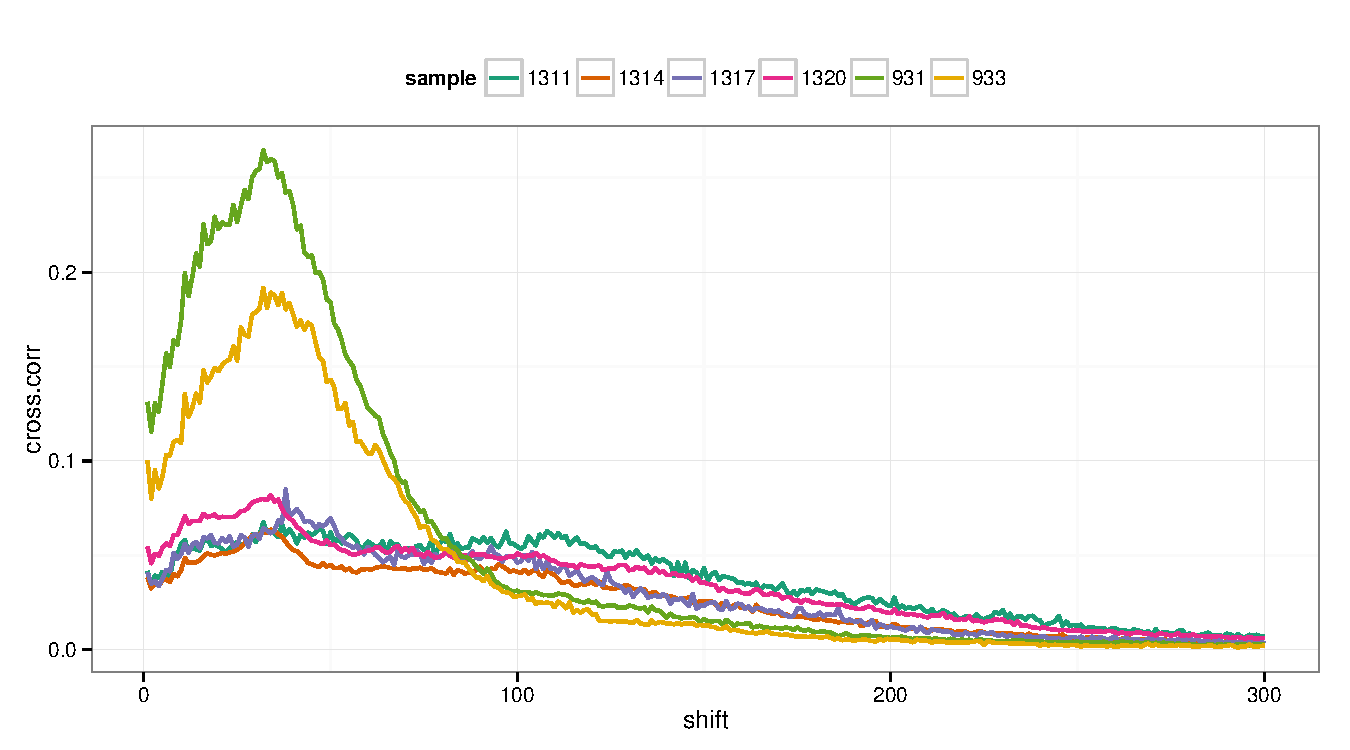
\includegraphics[width = .8\textwidth]{/p/keles/ChIPexo/volume3/ChIPexo/figs/for_paper/EColi_strand_cross_corr.pdf}
  \caption{SCC curves for $\sig$ samples. The ``phantom peak'' and the
    summit that corresponds to the read and fragment length
    respectively are confounded due to the exonuclease digestion.}
  \label{fig:scc_exo}
\end{figure}

\newpage

\begin{figure}[h!]
  \centering
  \includegraphics[width = .46\textwidth,page = 3 ]{../figs/for_paper/ChIPseqPET_ChIPexo_tagCount_comparison.pdf}
  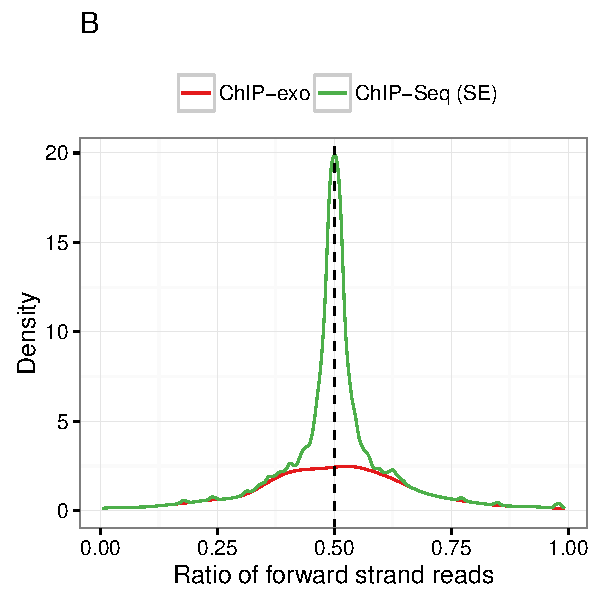
\includegraphics[width = .46\textwidth]{../figs/for_paper/forward_strand_ratio_comp_old.pdf}
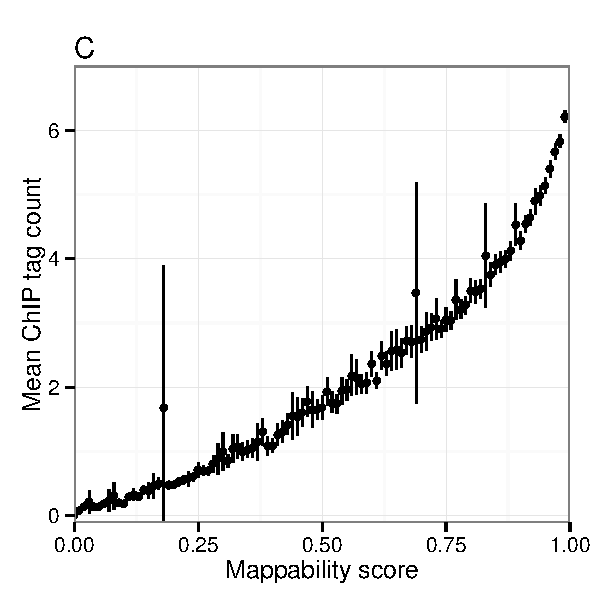
\includegraphics[width = .46\textwidth,page = 1]{../figs/for_paper/eukaryotic_bias_CTCF.pdf}
  \includegraphics[width = .46\textwidth,page = 2]{../figs/for_paper/eukaryotic_bias_CTCF.pdf}
  \caption{ A) Hexbin plot of PE ChIP-Seq bin counts VS ChIP-exo bin
    counts. B) Forward Strand Ratio densities for SE ChIP-Seq and
    ChIP-exo peaks. C) ChIP tag counts increase linearly as
    mappability scores increases. D) ChIP tag counts increase linearly
    as GC content score increases when GC content is less than 0.6 and
    then ChIP tag counts decrease as GC content increases. D)
    Percentage of sites with at least p.value.}
  \label{fig:comp}
\end{figure}

\newpage

\begin{figure}[h!]
  \centering
  \centering
  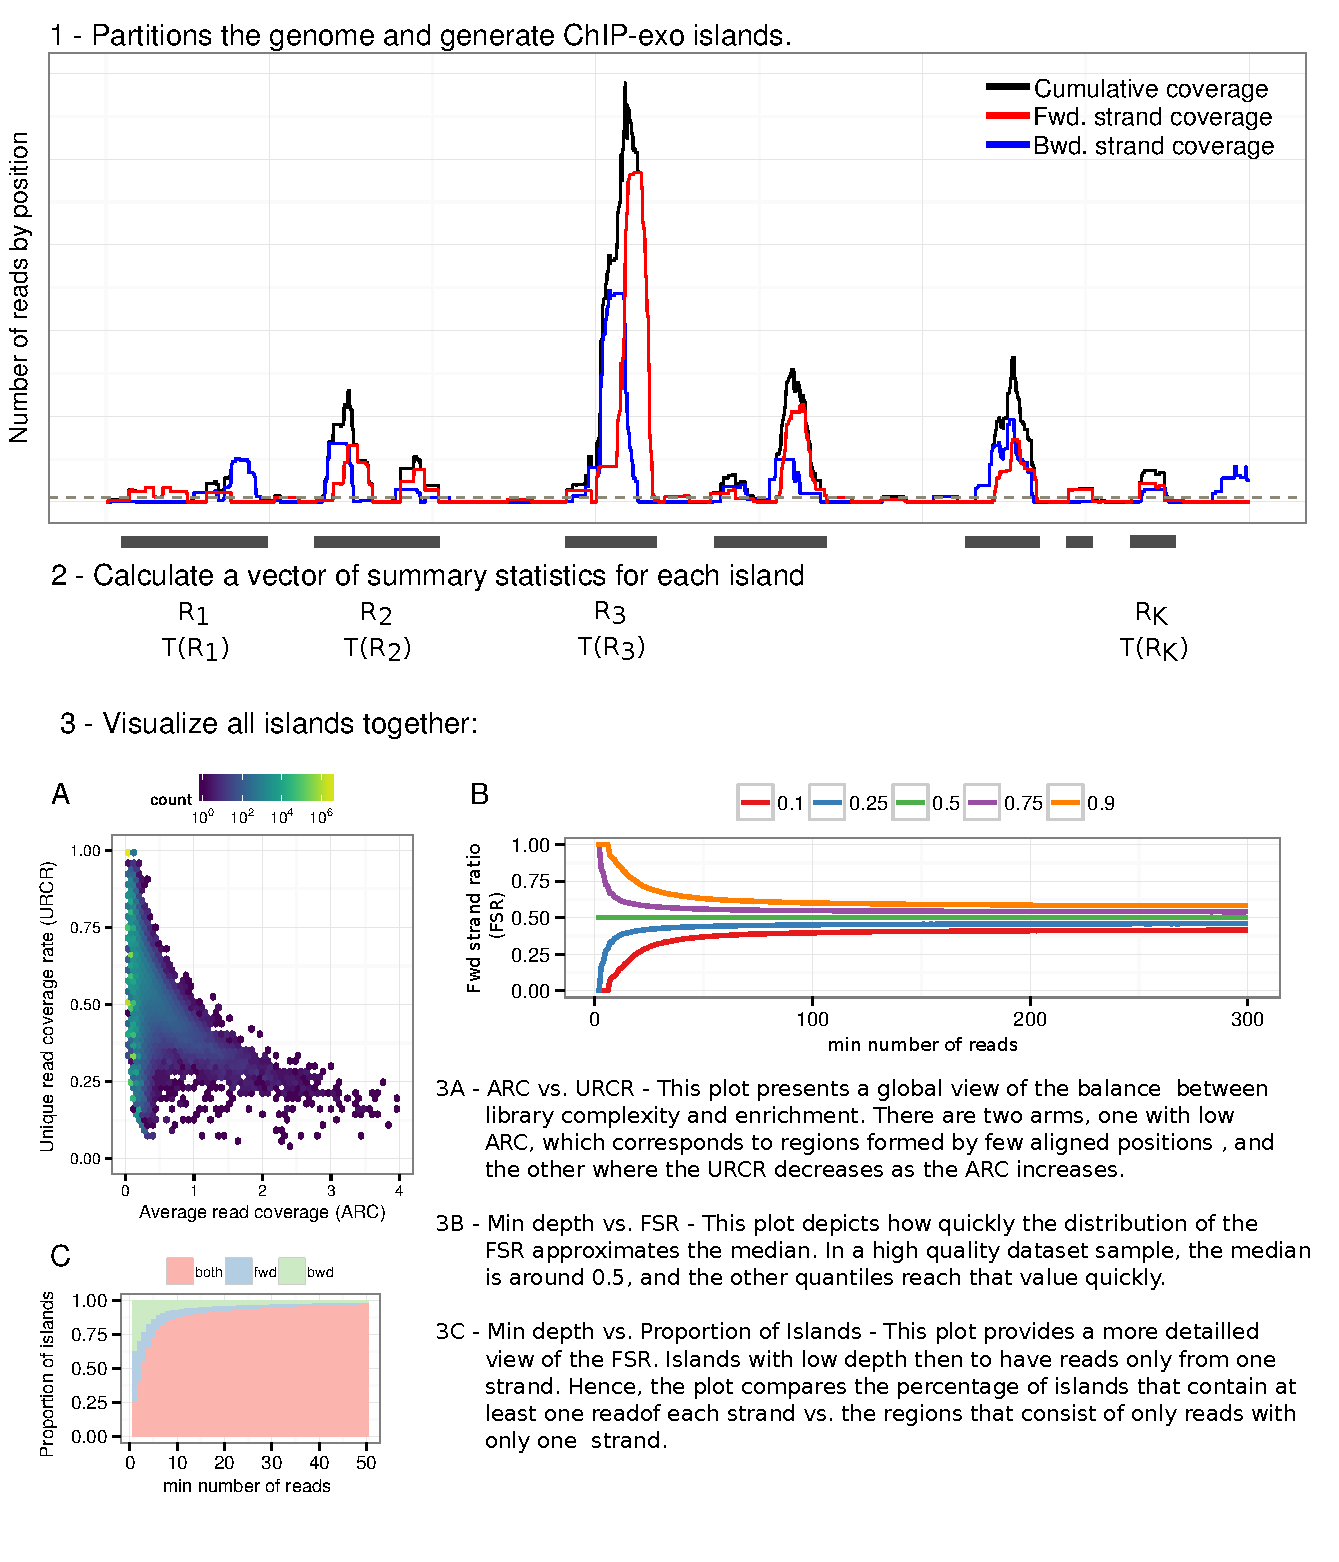
\includegraphics[width = \textwidth]{../figs/for_paper/coverage_diagram2.pdf}
  \caption{Flowchart of the ChIP-exo quality control pipeline.}
  \label{fig:qcdiagram}
\end{figure}

\newpage

\begin{figure}[h!]
  \centering
  \includegraphics[width = .9  \textwidth,page = 1]{../figs/Carroll_mice_for_paper/FoxA1_enrichment.pdf}
  \newline
  \includegraphics[width = .3 \textwidth,page = 1]{../figs/FOXA1_mm9_fimo/FOXA1_summaries_by_replicate.pdf}
  \includegraphics[width = .3 \textwidth,page = 3]{../figs/FOXA1_mm9_fimo/FOXA1_summaries_by_replicate.pdf}
  \includegraphics[width = .3 \textwidth,page = 1]{../figs/FOXA1_mm9_fimo/FOXA1_log10pval_cumulative_nmotifs.pdf}
  \caption{Using the mouse-FoxA1 experiment from \cite{exoillumina}:
    A) Hexbin plots of $\mbox{ARC}$ against $\mbox{URCR}$, in general
    we can see a slight separation into two strong arms, one
    corresponds to low $\mbox{ARC}$ and varying $\mbox{URCR}$, and for
    the other $\mbox{URCR}$ decreases as $\mbox{ARC}$ increases. B)
    Number of candidate sites for each replicate. C) Percentage of
    candidate sites where the FoxA1 motif was detected. D) 
 }
  \label{fig:enrich}
\end{figure}

\newpage

\begin{figure}[h!]
  \centering  
  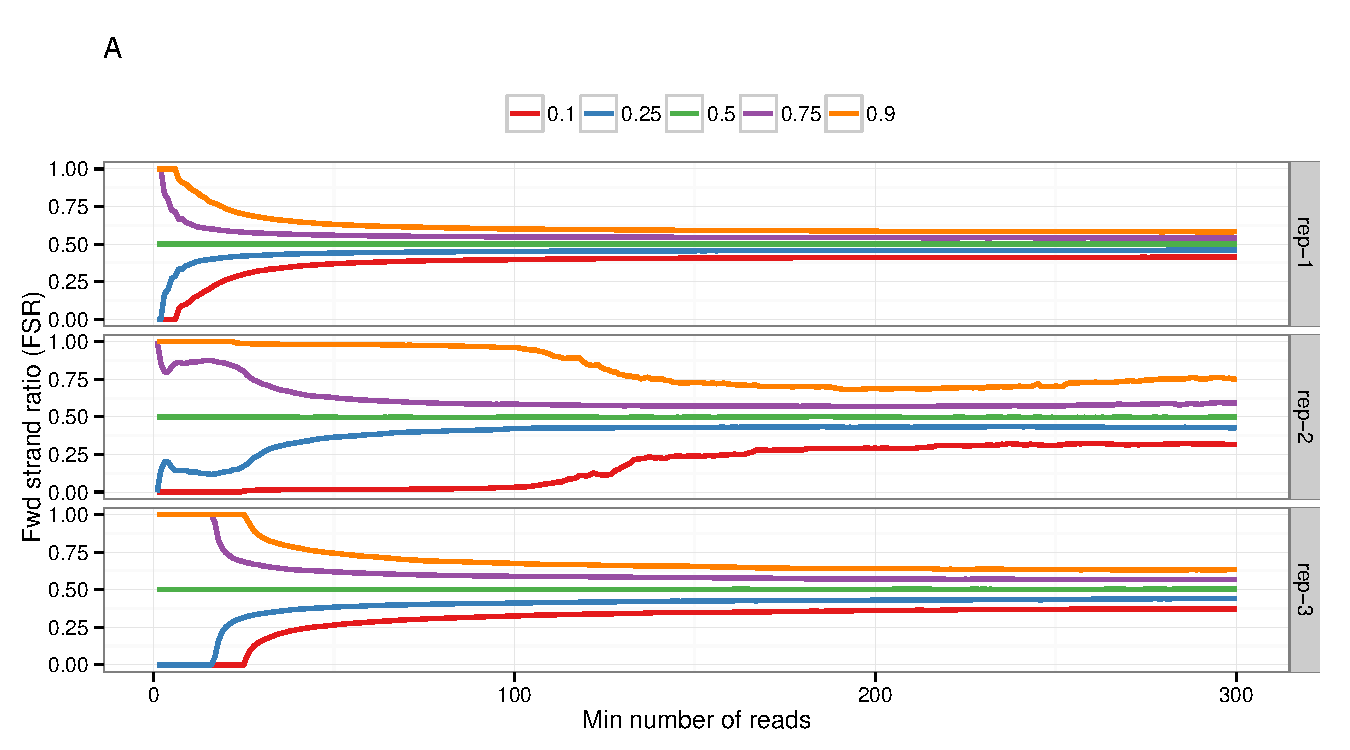
\includegraphics[width = .9\textwidth,page = 1]{../figs/Carroll_mice_for_paper/Strand_imbalance.pdf} 
  \newline
  \includegraphics[width = .9\textwidth,page = 2]{../figs/Carroll_mice_for_paper/Strand_imbalance.pdf} 
  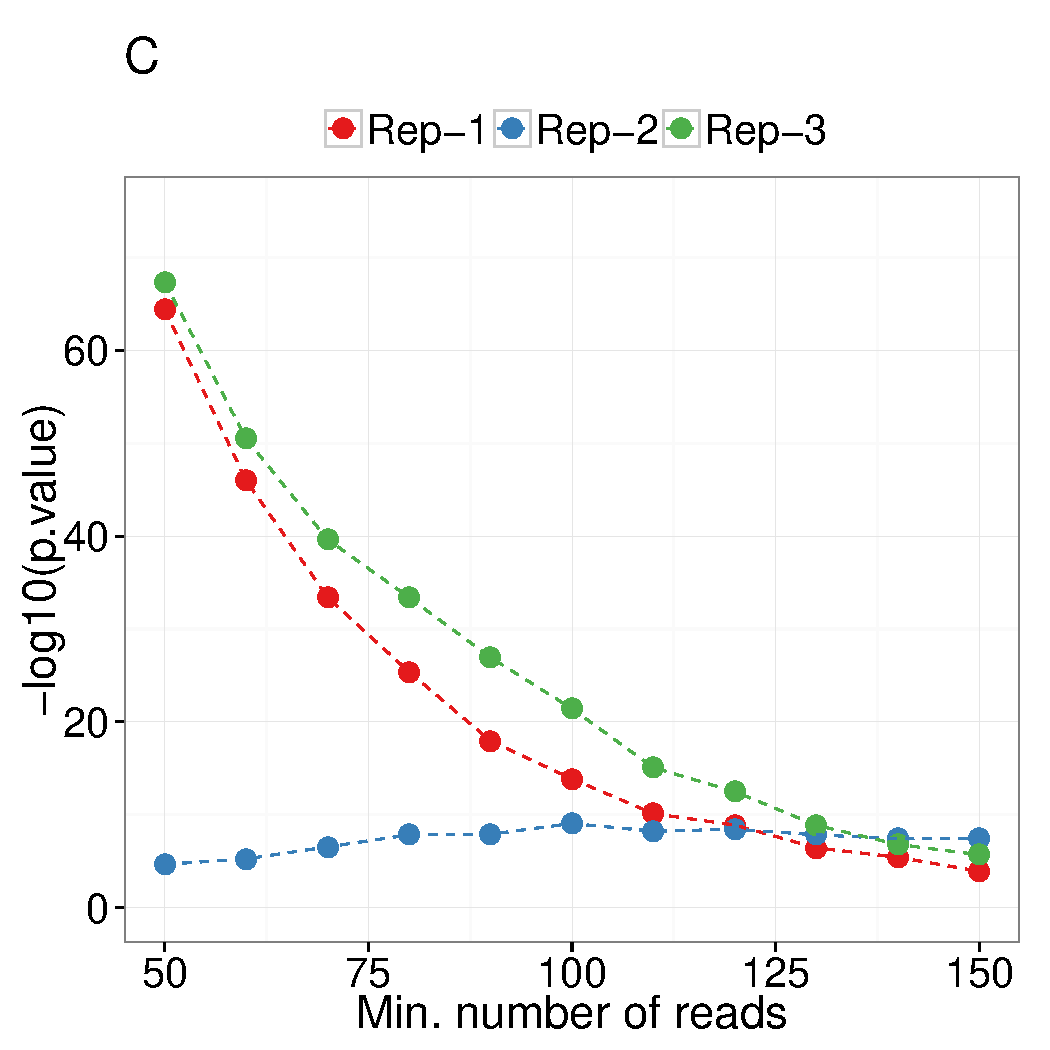
\includegraphics[width = .4\textwidth]{../figs/for_paper/Carroll_FSR_depth_VS_pvalWilcoxon.pdf}
  \caption{Strand imbalance QC plots for the same data as in Figure
    \ref{fig:enrich}A. A) FSR distribution quantiles as the lower
    depth regions are being filtered out, all quantiles approach to
    the median as the lower bound increases. B) Stacked histogram with
    the proportion of regions that are formed by two strands or only
    one, in a good sample the single-stranded regions are going to be
    filtered out quickly as in the middle row. C)
    $-log_{10}(\text{p.value})$ of testing if the imbalance
    distributions differs when ChIP-exo regions overlap their peaks.}
  \label{fig:strand}
\end{figure}

\newpage

\begin{figure}[h!]
  \centering
  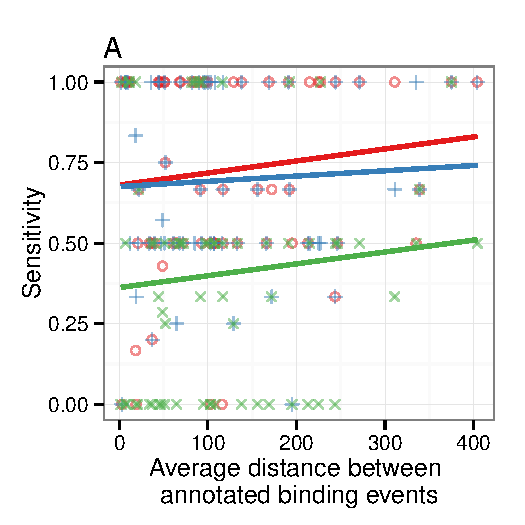
\includegraphics[width = .46\textwidth]{../figs/for_paper/sensitivity_exo_olda_data.pdf}
  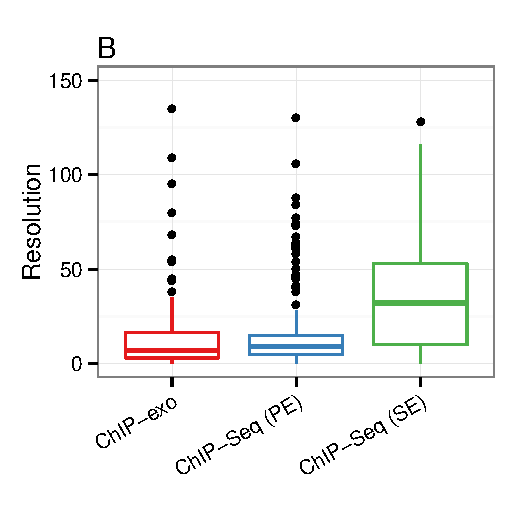
\includegraphics[width = .46\textwidth]{../figs/for_paper/resolution_by_dataset_old_data.pdf}
   \caption{Comparison of (A) sensitivity and (B) resolution between
     ChIP-exo and ChIP-Seq data. Sensitivity is defined as the
     proportion of RegulonDB annotations identified using each
     data. Resolution is defined as the distance between RegulonDB
     annotation and its closest prediction.}
  \label{fig:reso_all}
\end{figure}

\newpage

\begin{figure}[h]
  \centering
  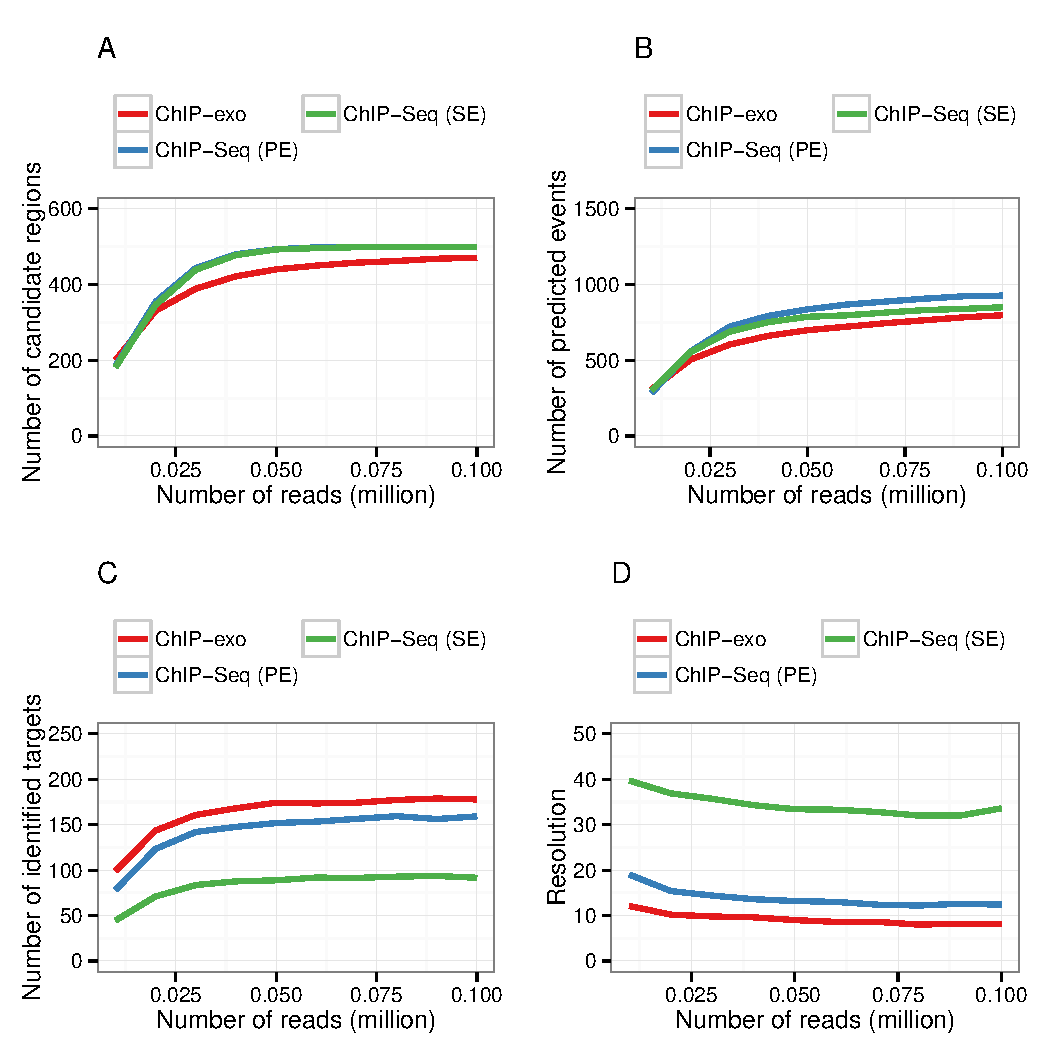
\includegraphics[width = .9\textwidth]{../figs/for_paper/saturation_analysis_old.pdf}
  \caption{Comparison of the number of candidate regions (A),
    predicted events (B), identified targets (C) and resolution (D)
    among ChIP-exo, PE ChIP-Seq and SE ChIP-Seq. RegulonDB annotations
    are considered as a gold standard. A gold standard binding events
    was deemed identified if a binding event was estimated at a $\pm$
    15 vicinity of it.}
  \label{fig:design}
\end{figure}


% \textbf{ChIP-exo, PE ChIP-Seq and SE ChIP-Seq comparison at varying
%   sequencing depths.} 
 \newpage

\begin{figure}[h!]
  \centering
\includegraphics[width = .9\textwidth]{../figs/saturation/K12_alignment/sig70_aerobic_enrichment.pdf}
\caption{Hexbin plots of ARC vs URCR of the $\sig$ ChIP-exo experiment
  under aerobic condition when 10K to 90K reads are being sampled.}
  \label{fig:exoQC_sat_aero}
\end{figure}

\newpage


\begin{figure}[h!]
  \centering
  \includegraphics[width = .9\textwidth]{../figs/for_paper/sig70_methods_comparison_FDR5_topM300.pdf}
  \caption{Comparison of the resolution between dPeak, Gem, Mace and
    Peakzilla methods. Resolution is defined as the minimum distance
    between a RegulonDB annotation an a predicted binding event.}
  \label{fig:methods_comp}
\end{figure}

\newpage

\section*{Supplement}
\label{sec:supp}


\begin{table}[h!]
%% need to fix format
  \centering
\begin{knitrout}
\definecolor{shadecolor}{rgb}{0.969, 0.969, 0.969}\color{fgcolor}\begin{kframe}
\begin{verbatim}
##                      files   nreads       pbc      nsc
## 1: edsn1396_Sig70.sort.bam 13445022 0.9426179 8.865244
## 2: edsn1398_Sig70.sort.bam 16538920 0.9378843 7.031836
## 3: edsn1400_Sig70.sort.bam 11642722 0.8891744 10.77284
## 4: edsn1402_Sig70.sort.bam 16854026 0.9407020 7.936239
## 5: edsn1396_Sig70.sort.bam  6722511 0.6632742  9.01779
## 6: edsn1398_Sig70.sort.bam  8269460 0.5594449 7.179539
## 7: edsn1400_Sig70.sort.bam  5821361 0.6472382 10.89898
## 8: edsn1402_Sig70.sort.bam  8427013 0.5895118 8.124717
\end{verbatim}
\end{kframe}
\end{knitrout}
\caption{Same QC metrics as in table \ref{tab:qc} but applied to
  Landick's chipseq data of the rif experiment}
\end{table}

\begin{figure}[h!]
  \centering % note change to stat_density(geom = "line")
   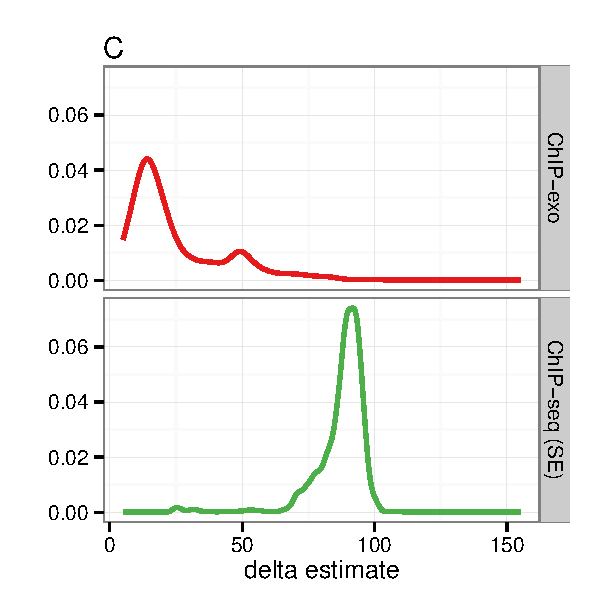
\includegraphics[width = .46\textwidth,page = 1]{../figs/for_paper/sigma_delta_old_densities.pdf}
   \includegraphics[width = .46\textwidth,page = 2]{../figs/for_paper/sigma_delta_old_densities.pdf}   
  \caption{ C) $\delta$ parameter in dPeak measures average distance
    of the reads to their respective binding site. In ChIP-exo data,
    reads were located much closer to the binding site than in SET
    ChIP-Seq. D) $\sigma$ parameter measure the dispersion of reads
    around each binding site. In ChIP-exo data, reads showed less
    variation around the their respective binding sites compared to
    SET ChIP-Seq.}

\end{figure}

\newpage

\begin{figure}[h!]
  \centering
  \includegraphics[width = .7\textwidth]{../figs/saturation/K12_alignment/PBC_saturation.pdf}
  \caption{Average PBC (among all seeds) of the sampled ChIP-exo, PE
    ChIP-Seq and SE ChIP-Seq experiments under the rif treatment
    conditions used for saturation analysis.}
  \label{fig:pbc_saturation}
\end{figure}

\newpage

\begin{figure}[h!] %%% fix this plot as one ggplot, facet_grid(condition ~ variable,scales = "free_y")
  \centering
  \begin{itemize}
  \item Rep-1 and rif-0min:
  \end{itemize}
  \includegraphics[width = .3\textwidth,page =2]{../figs/saturation/K12_alignment/Sig70_rep1_rif0_saturation_analysis.pdf}
  \includegraphics[width = .3\textwidth,page =3]{../figs/saturation/K12_alignment/Sig70_rep1_rif0_saturation_analysis.pdf}
  \includegraphics[width = .3\textwidth,page =4]{../figs/saturation/K12_alignment/Sig70_rep1_rif0_saturation_analysis.pdf}

  \begin{itemize}
  \item Rep-1 and rif-20min:
  \end{itemize}

  \includegraphics[width = .3\textwidth,page =2]{../figs/saturation/K12_alignment/Sig70_rep1_rif20_saturation_analysis.pdf}
  \includegraphics[width = .3\textwidth,page =3]{../figs/saturation/K12_alignment/Sig70_rep1_rif20_saturation_analysis.pdf}
  \includegraphics[width = .3\textwidth,page =4]{../figs/saturation/K12_alignment/Sig70_rep1_rif20_saturation_analysis.pdf}

  \begin{itemize}
  \item Rep-2 and rif-0min:
  \end{itemize}

  \includegraphics[width = .3\textwidth,page =2]{../figs/saturation/K12_alignment/Sig70_rep2_rif0_saturation_analysis.pdf}
  \includegraphics[width = .3\textwidth,page =3]{../figs/saturation/K12_alignment/Sig70_rep2_rif0_saturation_analysis.pdf}
  \includegraphics[width = .3\textwidth,page =4]{../figs/saturation/K12_alignment/Sig70_rep2_rif0_saturation_analysis.pdf}

  \begin{itemize}
  \item Rep-2 and rif-20min:
  \end{itemize}

  \includegraphics[width = .3\textwidth,page =2]{../figs/saturation/K12_alignment/Sig70_rep2_rif20_saturation_analysis.pdf}
  \includegraphics[width = .3\textwidth,page =3]{../figs/saturation/K12_alignment/Sig70_rep2_rif20_saturation_analysis.pdf}
  \includegraphics[width = .3\textwidth,page =4]{../figs/saturation/K12_alignment/Sig70_rep2_rif20_saturation_analysis.pdf}
  \caption{Comparison of the number of predicted events (left),
    identified targets (middle) and resolution (right) among ChIP-exo,
    PE ChIP-Seq and SE ChIP-Seq. RegulonDB annotations are considered
    as gold standard. A RegulonDB binding events was deemed identified
    if a binding event was estimated at a $\pm$ 15 vicinity
    of it.}
  \label{fig:saturation_rif}
\end{figure}

% \textbf{ChIP-exo, PE ChIP-Seq and SE ChIP-Seq comparison at varying
%   sequencing depth} 

\newpage

\begin{figure}[h!]
  \centering
  \includegraphics[width = .9\textwidth,page = 1]{../figs/saturation/K12_alignment/sig70_rif_enrichment.pdf}
  \caption{A) ARC vs URCR hexbin plots of Rep-1 and rif-0min from $\sig$ experiment when 100K to 900K reads are being
    sampled for each panel. }
  \label{fig:exoQC_sat1}
\end{figure}

\newpage

\begin{figure}[h!]
  \centering
  \includegraphics[width = .9\textwidth,page = 1]{../figs/saturation/K12_alignment/sig70_rif_enrichment.pdf}

  \caption{ARC vs URCR hexbin plots of Rep-1 and rif-20min from $\sig$ experiment when 100K to 900K reads are being
    sampled for each panel.}
  \label{fig:exoQC_sat2}
\end{figure}

\newpage

\begin{figure}[h!]
  \centering
  \includegraphics[width = .9\textwidth,page = 1]{../figs/saturation/K12_alignment/sig70_rif_enrichment.pdf}
  \caption{ARC vs URCR hexbin plots of Rep-2 and rif-0min from $\sig$ experiment when 100K to 900K reads are being
    sampled for each panel.}
  \label{fig:exoQC_sat3}
\end{figure}

\newpage

\begin{figure}[h!]
  \centering
  \includegraphics[width = .9\textwidth,page = 1]{../figs/saturation/K12_alignment/sig70_rif_enrichment.pdf}
  \caption{ARC vs URCR hexbin plots of Rep-2 and rif-20min from $\sig$ experiment when 100K to 900K reads are being
    sampled for each panel.}
  \label{fig:exoQC_sat4}
\end{figure}

\newpage




% \nocite{exo_gb}
%  \nocite{maplot1}
% \nocite{maplot2}
% \nocite{chipbeyond}
% \nocite{esl}


\end{document}

